\documentclass[12pt,fleqn]{examtst}
\usepackage{graphicx}
\usepackage{amssymb}
\usepackage{amsmath}
\usepackage{listings}
\usepackage{multirow}
\usepackage{multicol}
\usepackage{hhline}
\usepackage{booktabs}
\usepackage{url}
\usepackage{enumerate}
\usepackage{hyperref}
%% Comments

\usepackage{color}

\newif\ifcomments\commentstrue

\ifcomments
\newcommand{\authornote}[3]{\textcolor{#1}{[#3 ---#2]}}
\newcommand{\todo}[1]{\textcolor{red}{[TODO: #1]}}
\else
\newcommand{\authornote}[3]{}
\newcommand{\todo}[1]{}
\fi

\newcommand{\wss}[1]{\authornote{blue}{SS}{#1}}

\begin{document}

\newcommand{\soln}{n} %y for yes and n for no

\lstset{language=python, basicstyle=\ttfamily, breaklines=true,
  showspaces=false, showstringspaces=false, breakatwhitespace=true}

\newcommand{\codeit}[1]{\texttt{\textit{#1}}}

\begin{center}
  {\large \bf COMP SCI 2ME3 and SFWR ENG 2AA4 Midterm Examination}\\[1ex]
  {\large \bf McMaster University}\\[1ex]
  \ifthenelse{\equal{\soln}{y}}{\large {\bf ANSWER KEY} %Large arrow
    %($\Longleftarrow$) for correct% , small ($\leftarrow$) for partially
    % correct
  }{}
\end{center}

\medskip

\noindent
DAY CLASS%, \textbf{Version 1}
\hfill Dr.~S.~Smith \\
DURATION OF EXAMINATION: 3 hours \\
MCMASTER UNIVERSITY MIDTERM EXAMINATION \hfill March 4, 2021

\medskip

\noindent
\rule[3 mm]{\textwidth}{0.5mm}

%\begin{minipage}[t]{1.0\textwidth}

NAME: \wss{Cassidy Baldin}\\[1ex]

Student ID: \wss{400251130} \\[2mm]

\noindent
\rule[3 mm]{\textwidth}{0.5mm}

This examination paper includes \noofpages pages and
4 % VARIABILITY
questions. You are responsible for ensuring that your copy of the examination
paper is complete. Bring any discrepancy to the attention
of your instructor.\\

\noindent
\emph{By submitting this work, I certify that the work represents solely my own
independent efforts. I confirm that I am expected to exhibit honesty and use
ethical behavior in all aspects of the learning process.  I confirm that it is
my responsibility to understand what constitutes academic dishonesty under the
\href{https://secretariat.mcmaster.ca/app/uploads/Academic-Integrity-Policy-1-1.pdf}
{Academic Integrity Policy}}.\\

\noindent
\textbf{Special Instructions}:

\begin{enumerate}

\item For taking tests remotely: 
\begin{itemize}
\item Turn off all unnecessary programs, especially Netflix, YouTube, games like
  Xbox or PS4, anything that might be downloading or streaming.
\item If your house is shared, ask others to refrain from doing those activities
  during the test.
\item If you can, connect to the internet via a wired connection.
\item Move close to the Wi-Fi hub in your house. 
\item Restart your computer, 1-2 hours before the exam. A restart can be very
  helpful for several computer hiccups.
\item Commit and push your tex file, compiled pdf file, and code files
  frequently.
\item Ensure that you push your solution (tex file, pdf file and code files)
  before time expires on the test.  The solution that is in the repo at the
  deadline is the solution that will be graded.
\end{itemize}
\item It is your responsibility to ensure that the answer sheet is properly
  completed. Your examination result depends upon proper attention to the
  instructions.
\item All physical external resources are permitted, including textbooks, calculators,
  computers, compilers, and the internet.
\item The work has to be completed individually.  Discussion with others is
  strictly prohibited.
\item Read each question carefully.
\item Try to allocate your time sensibly and divide it appropriately between the
  questions.
\item The set $\mathbb{N}$ is assumed to include $0$.
\end{enumerate}
%\end{minipage}\\

\examheader{CS2ME3/SE2AA4 \ifthenelse{\equal{\soln}{y}} {\hfill SOLUTIONS} }

\renewcommand{\labelenumi}{\Alph{enumi}.}

\newpage

%%%%%%%%%%%%%%%%%%%%%%%%%%%%%%%%%%%%%%%%%%%%%%%%%%%%%%%%%%%%%%%%%%%%%%

\question{6 marks} %tests software qualities - reusability?
Parnas advocates faking a rational design process as depicted in the figure below.
The faked documentation follows these steps: Requirements (SRS) $\rightarrow$
Design (MG and MIS) $\rightarrow$ Application Implementation (code)
$\rightarrow$ Verification and Validation (Unit Testing, Integration Testing,
Review).  How are the principles of
a) abstraction and b) separation of concerns applied in a rational design
process?  In your answer you can refer to any aspects of the process,
documentation, and/or Parnas's principles.

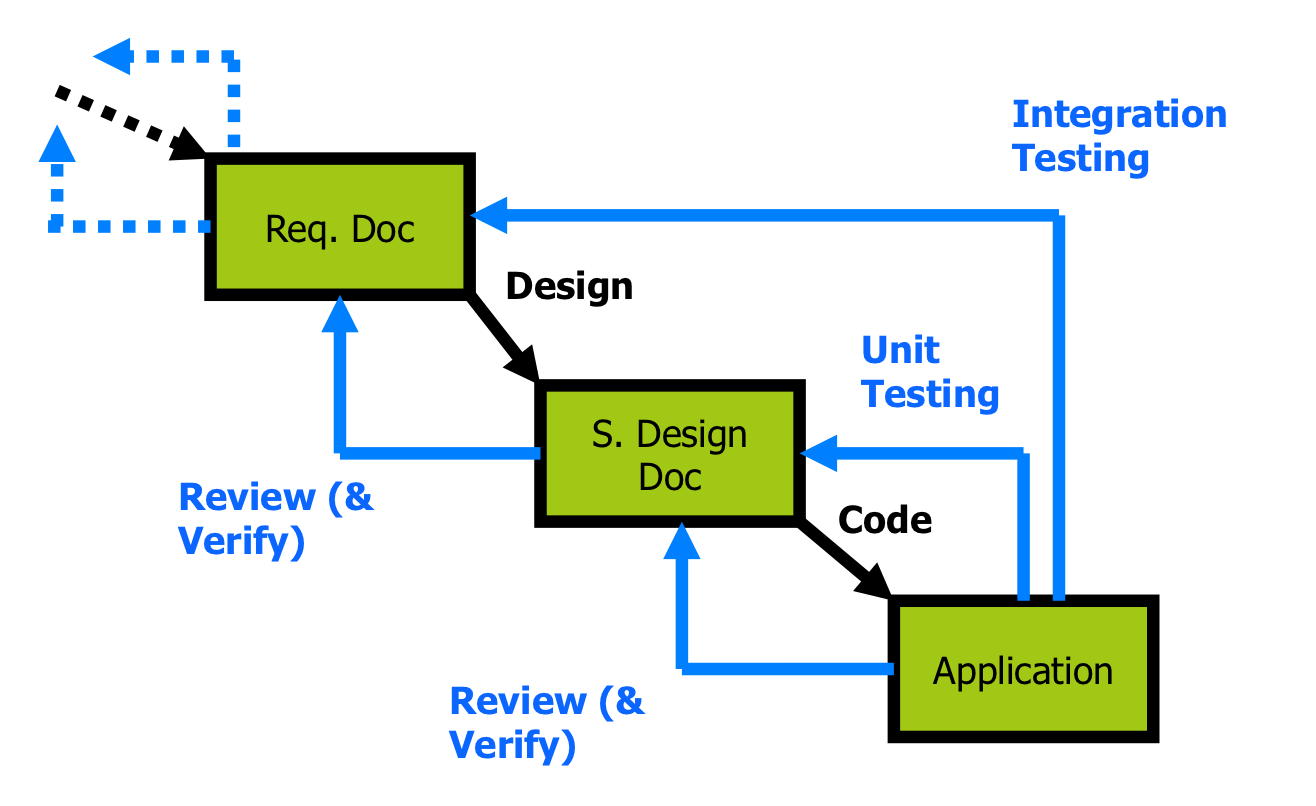
\includegraphics[scale=0.4]{SoftwareLifecycle.png}

\noindent \wss{Fill in your answer below}

\begin{enumerate}[a)]
\item Abstraction
  
The principle of abstraction is defined as the process of focusing on what is important while ignoring what is irrelevant in the project. This is also known as a special case of the principle of separation of concerns as will be explained later. This principle can be applied in a rational design process as you can use it to plan out what you are going to design/create before you actually start designing it, and allows you to take a look at the problem in a more abstract way. For example, when you are in the first stage of the faked rational design process which is “Requirements”, you can use this principle to look at these requirements in terms of what is most important so that you can start designing with those important details first, before worrying about the smaller things. This can allow designers to be able to make better decisions for the design, as they are more focused on what is crucial to the project, rather than getting lost in the small details that may not matter as much in the grand scheme of things. This principle can also be helpful in the design stage, as using an abstract mindset, you can make your design able to be used in many different ways or have many differing ideas brought about because you have taken the problem and instead of looking at it in a specific sense only as it might have constrained the design process.

\item Separation of Concerns

The principle of separation of concerns is defined as the principle that different concerns should be isolated and considered separately from one another. This principle can be applied to the faked rational design process as you can allow designers to reduce the problem from a complex and hard to grasp problem, to many simpler and easy to work with tasks. Since different concerns are considered at different times, in  the implementation step of this process, this can allow programmers to be able to split the problem into more parts that are simpler to work on and that can allow for easier work between people to occur, allowing for efficient work flow in solving the tasks at hand. This principle can also be helpful when documenting requirements of a design, as this can allow you to approach the problem in a more systematic way, separating some parts from others to focus on what it is that you need to accomplish and in what order. This can make planning and scheduling easier as well, as if the project is broken up into different parts, and each part can be estimated on how long it will take and what needs to be done to complete each task, this can help the people working on the project to get things done more efficiently. 

This is how the principles of abstraction and separation of concerns can be applied in a rational design process. 

\end{enumerate}

%%%%%%%%%%%%%%%%%%%%%%%%%%%%%%%%%%%%%%%%%%%%%%%%%%%%%%%%%%%%%%%%%%%%%%

\newpage

\noindent Consider the specification for two modules: SeqServices and SetOfInt.

\section* {Sequence Services Library}

\subsection*{Module}

SeqServicesLibrary

\subsection* {Uses}

None

\subsection* {Syntax}

\subsubsection* {Exported Constants}

None

\subsubsection* {Exported Types}

None 

\subsubsection* {Exported Access Programs}

\begin{tabular}{| l | l | l | p{5cm} |}
\hline
\textbf{Routine name} & \textbf{In} & \textbf{Out} & \textbf{Exceptions}\\
\hline
max\_val & seq of $\mathbb{Z}$ & $\mathbb{N}$ & ValueError\\
  \hline
count & $\mathbb{Z}$, seq of $\mathbb{Z}$ & $\mathbb{N}$ & ValueError\\
\hline
spices & seq of $\mathbb{Z}$ & seq of string & ValueError\\
\hline
new\_max\_val & seq of $\mathbb{Z}$, $\mathbb{Z} \rightarrow \mathbb{B}$ &
                                                                           $\mathbb{N}$ & ValueError\\
\hline
  
\end{tabular}

\subsection* {Semantics}

\subsubsection* {State Variables}

None

\subsubsection* {State Invariant}

None

\subsubsection* {Assumptions}

\begin{itemize}
\item All access programs will have inputs provided that match the types
  given in the specification.
\end{itemize}

\subsubsection* {Access Routine Semantics}

\noindent max\_val($s$)
\begin{itemize}
\item output: $\mathit{out} := | m |: \mathbb{N} \text{ such that } (m \in s) \wedge
  \forall (x: \mathbb{Z} | x \in s : | m | \geq | x |)$
\item exception: $(|s| = 0 \Rightarrow \text{ValueError})$
\end{itemize}

\noindent count($t, s$)
\begin{itemize}
\item output: $\mathit{out} := + (x: \mathbb{Z} | x \in s \wedge x = t : 1)$
\item exception: $(|s| = 0 \Rightarrow \text{ValueError})$
\end{itemize}

\noindent spices($s$)
\begin{itemize}
\item output: $\mathit{out} := \langle x: \mathbb{Z} | x \in s : (x \leq 0
  \Rightarrow \text{``nutmeg"} | \text{True} \Rightarrow \text{``ginger"}) \rangle$
\item exception: $(|s| = 0 \Rightarrow \text{ValueError})$
\end{itemize}

\noindent new\_max\_val($s$, $f$)
\begin{itemize}
\item output: $\mathit{out} := \text{max\_val}(\langle x: \mathbb{Z} | x \in s
  \wedge f(x): x \rangle )$
\item exception: $(|s| = 0 \Rightarrow \text{ValueError})$
\end{itemize}

%%%%%%%%%%%%%%%%%%%%%%%%%%%%%%%%%%

\newpage

\section* {Set of Integers Abstract Data Type}

\subsection* {Template Module}

SetOfInt

\subsection* {Uses}

None

\subsection* {Syntax}

\subsubsection* {Exported Types}

SetOfInt = ?

\subsubsection* {Exported Constants}

None

\subsubsection* {Exported Access Programs}

\begin{tabular}{| l | l | l | p{6cm} |}
\hline
\textbf{Routine name} & \textbf{In} & \textbf{Out} & \textbf{Exceptions}\\
\hline
new SetOfInt & seq of $\mathbb{Z}$ & SetOfInt & \\
\hline
is\_member & $\mathbb{Z}$ & $\mathbb{B}$ & \\
\hline
to\_seq &  & seq of $\mathbb{Z}$ & \\
\hline
union & SetOfInt & SetOfInt & \\
\hline
diff & SetOfInt & SetOfInt & \\
\hline
size &  & $\mathbb{N}$ & \\
\hline
empty &  & $\mathbb{B}$ & \\
\hline
equals & SetOfInt & $\mathbb{B}$ & \\
\hline

\end{tabular}

\subsection* {Semantics}

\subsubsection* {State Variables}

$s$: set of $\mathbb{Z}$

\subsubsection* {State Invariant}

None

\subsubsection* {Assumptions}

\begin{itemize}
\item The SetOfInt constructor is called for each object instance before any
  other access routine is called for that object.  The constructor can only be
  called once.  All access programs will have inputs provided that match the types
  given in the specification.
\end{itemize}

\subsubsection* {Access Routine Semantics}

\noindent new SetOfInt($x_s$):
\begin{itemize}
\item transition: $s := \cup (x: \mathbb{Z} | x \in x_s : \{ x \} )$
\item output: $\mathit{out} := \mathit{self}$
\item exception: none
\end{itemize}

\noindent is\_member($x$):
\begin{itemize}
\item output: $x \in s$
\item exception: none
\end{itemize}

\noindent to\_seq():
\begin{itemize}
\item output: $out := \mbox{set\_to\_seq}(s)$
\item exception: none
\end{itemize}

\noindent union($t$):
\begin{itemize}
\item output: $\text{SetOfInt} (\mbox{set\_to\_seq}(s) ||
  t.\text{to\_seq()})$

  \textit{\# in case it is clearer, an alternate version of output is:}
  
  $\text{SetOfInt}(\text{set\_to\_seq}(s \cup \{x: \mathbb{Z} | x \in t.\text{to\_seq()} : x \}))$
  
\item exception: none
\end{itemize}

\noindent diff($t$):
\begin{itemize}
\item output:
  $\text{SetOfInt}( \text{set\_to\_seq} (s \cap \text{complement}(t.\text{to\_seq()})))$
  
\item exception: none
\end{itemize}

\noindent size():
\begin{itemize}
\item output: $| s |$
\item exception: none
\end{itemize}

\noindent empty():
\begin{itemize}
\item output: $s = \varnothing$
\item exception: none
\end{itemize}

\noindent equals($t$):
\begin{itemize}
\item output: $\forall ( x: \mathbb{Z} | x \in \mathbb{Z} : x \in
  t.\text{to\_seq()} \leftrightarrow x \in s)$ \textit{\# this means:} $t.\text{to\_seq}() = s$
\item exception: none
\end{itemize}

\subsection*{Local Functions}

\noindent $\mbox{set\_to\_seq}: \text{set of } \mathbb{Z} \rightarrow \mbox{seq of }
\mathbb{Z}$\\
\noindent
$\mbox{set\_to\_seq}(s) \equiv \langle x: \mathbb{Z} | x \in s : x \rangle$
\textit{\# Return a seq of all of the elems in the set s, order does not matter}\\

\noindent $\mbox{complement}: \text{seq of } \mathbb{Z} \rightarrow \mbox{ set of }
\mathbb{Z}$\\
$\mbox{complement}(A) \equiv \{ x: \mathbb{Z} | x \not\in A : x \}$\\

%%%%%%%%%%%%%%%%%%%%%%%%%%%%%%%%%%

\newpage

\noindent
\begin{minipage}{\textwidth}
\question{15 marks} \label{Q_PythonCode}

\wss{Complete Python code to match the above specification.}  The files you need
to complete are: \texttt{SeqServicesLibrary.py} and \texttt{SetOfInt.py}.  Two
testing files are also provided: \texttt{expt.py} and \texttt{test\_driver.py}.
The file \texttt{expt.py} is pre-populated with some simple experiments to help
you see the interface in use, and do some initial test.  You are free to add to
this file to experiment with your work, but the file itself isn't graded.  The
\texttt{test\_driver.py} is also not graded.  However, you may want to create
test cases to improve your confidence in your solution.  The stubs of the
necessary files are already available in your \texttt{src} folder.  The code
will automatically be imported into this document when the \texttt{tex} file is
compiled.  You should use the provided Makefile to test your code.  You will NOT
need to modify the Makefile.  The given Makefile will work for \texttt{make
  test}, without errors, from the initial state of your repo.  The \texttt{make
  expt} rule will also work, because all lines of code have been commented out.
Uncomment lines as you complete work on each part of the modules relevant to
those lines in \texttt{expt.py} file.  The required imports are already given in
the code.  You should not make any modifications in the provided import
statements.  You should not delete the ones that are already there.  Although
you can solve the problem without adding any imports, if your solution requires
additional imports, you can add them.  As usual, the final test is whether the
code runs on mills.

Any exceptions in the specification have names identical to the expected Python
exceptions; your code should use exactly the exception names as given in the
spec.

You do not need to worry about doxygen comments.  However, you should include
regular comments in the code where it would benefit from an explanation.

You do not need to worry about PEP8.  Adherence to PEP8 will not be part of the
grading.

Remember, your code needs to implement the given specification so that the
interface behaves as specified.  This does NOT mean that the local functions
need to all be implemented, or that the types used internally to the spec need
to be implemented exactly as given.  If you do implement any local functions,
please make them private by preceding the name with double underscores.\\

\end{minipage}

\newpage

\subsection*{Code for SeqServicesLibrary.py}

\noindent \lstinputlisting{./src/SeqServicesLibrary.py}

\newpage

\subsection*{Code for SetOfInt.py}

\noindent \lstinputlisting{./src/SetOfInt.py}

\newpage

\subsection*{Code for expt.py}

\noindent \lstinputlisting{./src/expt.py}

\newpage

\subsection*{Code for test\_driver.py}

\noindent \lstinputlisting{./src/test_driver.py}

\newpage

%%%%%%%%%%%%%%%%%%%%%%%%%%%%%%%%%%

\noindent
\begin{minipage}{\textwidth}
\question{5 marks} 

Critique the design of the interface for the SetOfInt module.  Specifically,
review the interface with respect to its consistency, essentiality, generality
and minimality.  Please be specific in your answer.

\wss{Put your answer for each quality below.}

\begin{itemize}
\item \textbf{consistency}:

The design for SetOfInt in terms of its consistency was indeed consistent in regards to implementation and use of its methods. Consistency is defined as the requirement that use of the same project carried out by different people using the same method should produce a similar result, meaning that if one person was to create and use a method from this specification, someone else should also get a similar result when doing it as well. This specification was consistent, as it used a more formal way of defining what each method was supposed to do in terms of math and its notation. Each method also showed the naming conventions, ordering of parameters, and exceptions that it needed to have, so that anyone who would implement this specification would be able to reproduce the same design, and therefore get the same results as someone else. There is slight room for error as some implementations of this specification might be different, but if they follow the specification, then they should expect to get the same results as another implementation. Therefore, this specification is consistent. 

\item \textbf{essentiality}:

The design for SetOfInt in terms of its essentiality was not essential, as it had methods that were redundant. A specification that is essential is defined as one that omits unnecessary features from a design so that it is the most useful it can be, without adding extra bulk to the design. In this specification, there are methods called \verb|size| and \verb|empty| where they return the size of the set and a boolean to tell if the set is empty respectively. The \verb|empty| method is not essential, as the \verb|size| method is already in place and can tell the user if the set is empty of not (if the size is zero it is empty). Therefore this interface as a whole is not essential, however the rest of the methods are unique making them essential methods. 

\item \textbf{generality}:

The design of SetOfInt in terms of its generality is not very general, as it is only dealing with sets of integers, as opposed to a more general solution to this problem that could deal with a set of any data type. Generality is defined as a way to generalize a solution to a given specific problem, so that it can be used not just for that one specific problem, but can be used to solve others as well. This allows a program to be reused for other purposes once the main problem has been solved. In the case of this specification, since it is only dealing with sets of integers, it cannot be generalized for sets of other data types like floats or strings, it that is not in the specification (or in the name which is very specific). This means that it would not be able to be used for many other purposes as this principle suggests, meaning it is not a very general specification. 

\item \textbf{minimality}:

The design of SetOfInt in terms of its minimality is indeed a minimal design as it contains unique access routines. A specification that is minimal avoids access routines with two or more potentially independent services (such as a getter that returns two state variables of the class). In the case of this specification, it is minimal as each method serves one purpose and only returns one value or object, meaning that this design is minimal. 

\end{itemize}

\end{minipage}

%%%%%%%%%%%%%%%%%%%%%%%%%%%%%%%%%%

\newpage

\noindent
\begin{minipage}{\textwidth}
\question{4 marks}

The module SetOfInt is for a set of integers.  Please answer the following
questions related to making that module generic. 
\begin{enumerate}[a.]
\item How would you change the specification to make it generic?  (Specifically
  what changes would you make to the given specification.  You don't need to
  redo the spec, just summarize what changes you would need to make.)
\item What changes would you need to make to the Python
implementation to make it generic for type T?  (Again, you can describe and
characterize the changes; you don't actually have to make them.)
\item What relational operator needs to be defined for type T to be a valid
  choice?
\item BONUS (1 mark) How would you specify (in the MIS) the relational operator
  constraint (from the previous question) on the generic type T?
\end{enumerate}

\wss{Put your answer below.}

\begin{enumerate}[a.]
\item 

The changes I would make to make this specification more generic would be to change the types of values that the methods take into the class (and change the name too). For example the specification only takes in integer values in the set in the constructor. In order to make this more generic, instead of only making it take in integer values in the set, it could take in floats, strings etc, so that it could be used to perform operations of sets for all data types. This would make it more generic as it would allow this specification to be used for many other applications, rather than strictly for applications involving integers in a set. 

\item

The changes I would need to make to the Python implementation to make it generic for inputs of type T would be to change the \verb|equals| method to account for differing types of inputs. This could be using an exception case or an if statement to catch if this is the case, and to stop any errors from occurring as a result. The rest of the design specification seems to already account for this generic change however, as it iterates through each set in terms of its length, and does not compare the exact values until the \verb|equals| method. 

\item

The relational operator that needs to be defined for type T to be a valid choice is the equal to operator, as the \verb|equals| method is the only method that might be affected by this change from type integer to type T (as it is the only access routine that uses a relational operator). This needs to be defined as if this specification was to be used for sets of multiple types (ex. floats and strings), this would be a problem in the current implementation, as when it tries to compare the two sets, it may throw an error as the two sets are not of the same type. This could be handled 

\item (BONUS)

In the MIS you could specify the relational operator constraint by adding an exception in the \verb|equals| method to check for whether the two sets being compared are of the same type. This would not allow sets that are not of the same type to be compared. This could also be changed by a conditional statement in the MIS in the \verb|equals| method where if the input set is of a different type from the other set, it will return False, as there is no way for the two sets to be equal if the both involve different data types. This could be done by checking the type first before doing the comparison. 

\end{enumerate}

\end{minipage}

\end{document}